% Practice Test 11 — Virginia Edition
% Questions: 30 (19 MC + 11 SA)
% Generated by scripts/generate_practice_tests.py

\begin{practiceQuestion}{1-4-q09}{mc}
\begin{questionText}
Lily earns $\$12.50$ per hour. She wants to buy a $\$75$ skateboard. Which equation can she use to find how many hours $h$ she needs to work?
\end{questionText}
\choiceA{$75 = 12.50 + h$}
\choiceB{$12.50 = 75h$}
\choiceC{$75 = 12.50h$}
\choiceD{$h = 75 + 12.50$}
\correctAnswer{C}
\explanation{Earnings $= 12.50 \times$ hours. Set earnings equal to $\$75$: $75 = 12.50h$.}
\end{practiceQuestion}

\begin{practiceQuestion}{2-1-q11}{mc}
\begin{questionText}
A baker made $120$ cupcakes and sold $90$ of them. What percent of the cupcakes were sold?
\end{questionText}
\choiceA{$60\%$}
\choiceB{$70\%$}
\choiceC{$75\%$}
\choiceD{$80\%$}
\correctAnswer{C}
\explanation{Divide: $90 \div 120 = 0.75 = 75\%$.}
\end{practiceQuestion}

\begin{practiceQuestion}{2-2-q13}{mc}
\begin{questionText}
A town has $2{,}400$ households. A survey shows $78\%$ have internet access. How many households have internet?
\end{questionText}
\choiceA{$1{,}800$}
\choiceB{$1{,}848$}
\choiceC{$1{,}872$}
\choiceD{$1{,}920$}
\correctAnswer{C}
\explanation{$\frac{n}{2400} = \frac{78}{100}$. Cross-multiply: $100n = 187{,}200$. Divide: $n = 1{,}872$.}
\end{practiceQuestion}

\begin{practiceQuestion}{2-3-q08}{mc}
\begin{questionText}
A computer originally costs $\$600$. After a $15\%$ price drop, what is the new price?
\end{questionText}
\choiceA{$\$90$}
\choiceB{$\$510$}
\choiceC{$\$515$}
\choiceD{$\$585$}
\correctAnswer{B}
\explanation{Multiply by $1 - 0.15 = 0.85$: $600 \times 0.85 = \$510$.}
\end{practiceQuestion}

\begin{practiceQuestion}{2-7-q03}{mc}
\begin{questionText}
In the percent error formula, why do we use absolute value?
\end{questionText}
\choiceA{To make the calculation easier}
\choiceB{Because the answer must be positive}
\choiceC{Because we only care about the size of the error, not the direction}
\choiceD{To convert the answer to a percent}
\correctAnswer{C}
\explanation{Absolute value ensures the percent error is positive whether the estimate was too high or too low.}
\end{practiceQuestion}

\begin{practiceQuestion}{3-2-q09}{mc}
\begin{questionText}
A diver is at $-20$ feet. She rises $8$ feet. What is her new depth?
\end{questionText}
\choiceA{$-28$ feet}
\choiceB{$-12$ feet}
\choiceC{$12$ feet}
\choiceD{$28$ feet}
\correctAnswer{B}
\explanation{$(-20) + 8 = -12$. Rising from a negative position adds a positive: $20 - 8 = 12$, keep negative.}
\end{practiceQuestion}

\begin{practiceQuestion}{3-3-q09}{mc}
\begin{questionText}
Which problem has the greatest answer?
\end{questionText}
\choiceA{$5 - 12$}
\choiceB{$(-3) - (-10)$}
\choiceC{$(-8) - 1$}
\choiceD{$2 - 7$}
\correctAnswer{B}
\explanation{A: $5 - 12 = -7$. B: $(-3) + 10 = 7$. C: $(-8) + (-1) = -9$. D: $2 - 7 = -5$. The greatest is $7$.}
\end{practiceQuestion}

\begin{practiceQuestion}{3-4-q08}{mc}
\begin{questionText}
A diver is at $-12.5$ meters. She rises $4.8$ meters. What is her new depth?
\end{questionText}
\choiceA{$-17.3$ m}
\choiceB{$-7.7$ m}
\choiceC{$7.7$ m}
\choiceD{$-8.3$ m}
\correctAnswer{B}
\explanation{$-12.5 + 4.8 = -7.7$ m. Different signs: $12.5 - 4.8 = 7.7$, keep negative.}
\end{practiceQuestion}

\begin{practiceQuestion}{4-3-q27}{gmc}
\begin{questionText}
The area model shows a rectangle split into two parts. What is the expanded form?

\begin{center}
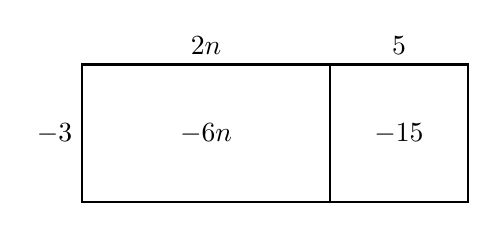
\begin{tikzpicture}[scale=0.7]
  \draw[thick] (0,0) rectangle (7,2.5);
  \draw[thick] (4.5,0) -- (4.5,2.5);
  \node[left] at (0,1.25) {$-3$};
  \node[above] at (2.25,2.5) {$2n$};
  \node[above] at (5.75,2.5) {$5$};
  \node at (2.25,1.25) {$-6n$};
  \node at (5.75,1.25) {$-15$};
\end{tikzpicture}
\end{center}
\end{questionText}
\choiceA{$-3(2n + 5) = -6n + 15$}
\choiceB{$-3(2n + 5) = -6n - 15$}
\choiceC{$-3(2n - 5) = -6n - 15$}
\choiceD{$3(2n + 5) = 6n + 15$}
\correctAnswer{B}
\explanation{The height is $-3$ and the width splits into $2n$ and $5$. Products: $-3 \times 2n = -6n$ and $-3 \times 5 = -15$. So $-3(2n + 5) = -6n - 15$.}
\end{practiceQuestion}

\begin{practiceQuestion}{4-4-q30}{gsa}
\begin{questionText}
A store sells gift boxes. The cost for $n$ gift boxes and $n$ greeting cards is shown below. Factor the total cost completely.

\begin{center}
\begin{tabular}{|c|c|c|}
\hline
\textbf{Item} & \textbf{Price Each} & \textbf{Quantity} \\
\hline
Gift box & $\$6$ & $n$ \\
\hline
Greeting card & $\$3$ & $n$ \\
\hline
\multicolumn{2}{|c|}{\textbf{Total Cost}} & $6n + 3n$ \\
\hline
\end{tabular}
\end{center}
\end{questionText}
\correctAnswer{$3n(2 + 1) = 3n(3) = 9n$, or factored as $3n(2 + 1)$}
\explanation{Total cost $= 6n + 3n$. The GCF is $3n$. Factor: $6n \div 3n = 2$ and $3n \div 3n = 1$. So $6n + 3n = 3n(2 + 1) = 3n \times 3 = 9n$.}
\end{practiceQuestion}

\begin{practiceQuestion}{5-4-q22}{sa}
\begin{questionText}
Solve $-0.3x + 4.2 = 1.8$.
\end{questionText}
\correctAnswer{$x = 8$}
\explanation{Subtract $4.2$: $-0.3x = -2.4$. Divide by $-0.3$: $x = 8$. Check: $-0.3(8) + 4.2 = -2.4 + 4.2 = 1.8$ \checkmark.}
\end{practiceQuestion}

\begin{practiceQuestion}{5-5-q16}{mc}
\begin{questionText}
Solve $\dfrac{n}{5} - 2 > 4$.
\end{questionText}
\choiceA{$n > 10$}
\choiceB{$n > 30$}
\choiceC{$n > 1$}
\choiceD{$n < 30$}
\correctAnswer{B}
\explanation{Add $2$: $\frac{n}{5} > 6$. Multiply by $5$: $n > 30$.}
\end{practiceQuestion}

\begin{practiceQuestion}{5-6-q04}{mc}
\begin{questionText}
Solve $3n - 6 > 0$ and describe the graph.
\end{questionText}
\choiceA{Closed circle at $2$, shade right}
\choiceB{Open circle at $2$, shade right}
\choiceC{Open circle at $2$, shade left}
\choiceD{Closed circle at $-2$, shade right}
\correctAnswer{B}
\explanation{Add $6$: $3n > 6$. Divide by $3$: $n > 2$. Open circle at $2$, shade right.}
\end{practiceQuestion}

\begin{practiceQuestion}{6-1-q14}{mc}
\begin{questionText}
If the scale factor of a drawing is $5$, and the drawing area of a room is $8$ cm$^2$, what is the actual area?
\end{questionText}
\choiceA{$40$ m$^2$}
\choiceB{$200$ m$^2$}
\choiceC{$200$ cm$^2$}
\choiceD{$25$ cm$^2$}
\correctAnswer{C}
\explanation{Area scales by $k^2 = 5^2 = 25$. Actual area in drawing units: $8 \times 25 = 200$ cm$^2$.}
\end{practiceQuestion}

\begin{practiceQuestion}{6-2-q20}{sa}
\begin{questionText}
A map uses $1$ cm $= 100$ km. You redraw at $1$ cm $= 25$ km. A distance is $3$ cm on the original. How long is it on the new map?
\end{questionText}
\correctAnswer{$12$ cm}
\explanation{Scale ratio: $\frac{100}{25} = 4$. New length: $3 \times 4 = 12$ cm.}
\end{practiceQuestion}

\begin{practiceQuestion}{6-5-q26}{gmc}
\begin{questionText}
The diagram shows a rectangular prism being sliced by a horizontal plane (dashed line). What is the cross-section?

\begin{center}
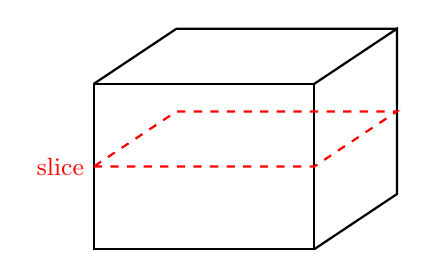
\begin{tikzpicture}[scale=0.7]
  % Rectangular prism
  \draw[thick] (0,0) -- (4,0) -- (4,3) -- (0,3) -- cycle; % front face
  \draw[thick] (4,0) -- (5.5,1) -- (5.5,4) -- (4,3); % right face
  \draw[thick] (0,3) -- (1.5,4) -- (5.5,4); % top face
  \draw[dashed,thick,red] (0,1.5) -- (4,1.5) -- (5.5,2.5) -- (1.5,2.5) -- cycle;
  \node[left,red] at (0,1.5) {\small slice};
\end{tikzpicture}
\end{center}
\end{questionText}
\choiceA{Triangle}
\choiceB{Rectangle}
\choiceC{Circle}
\choiceD{Trapezoid}
\correctAnswer{B}
\explanation{A horizontal slice through a rectangular prism always produces a rectangle congruent to the base.}
\end{practiceQuestion}

\begin{practiceQuestion}{6-6-q29}{gsa}
\begin{questionText}
Two lines intersect as shown. Find the values of $a$, $b$, and $c$.

\begin{center}
\begin{tikzpicture}[scale=0.8]
  \draw[thick] (-3,0) -- (3,0);
  \draw[thick] (-2,-2.5) -- (2,2.5);
  \node at (1.8,0.7) {\small $a°$};
  \node at (-1.8,0.7) {\small $b°$};
  \node at (-1.8,-0.8) {\small $c°$};
  \node at (1.8,-0.8) {\small $52°$};
\end{tikzpicture}
\end{center}
\end{questionText}
\correctAnswer{$a = 128°$, $b = 52°$, $c = 128°$}
\explanation{Vertical to $52°$: $b = 52°$. Supplementary to $52°$: $a = 180° - 52° = 128°$. Vertical to $a$: $c = 128°$.}
\end{practiceQuestion}

\begin{practiceQuestion}{6-7-q30}{gsa}
\begin{questionText}
The graph shows triangle $PQR$ with $P(2, 3)$, $Q(5, 3)$, and $R(5, 7)$. Rotate the triangle $90°$ clockwise about the origin. List the new vertices.

\begin{center}
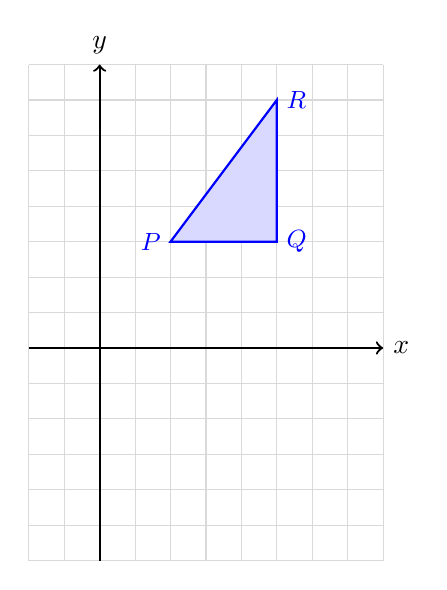
\begin{tikzpicture}[scale=0.45]
  \draw[step=1,gray!30,thin] (-2,-6) grid (8,8);
  \draw[thick,->] (-2,0) -- (8,0) node[right]{$x$};
  \draw[thick,->] (0,-6) -- (0,8) node[above]{$y$};
  \draw[thick,blue,fill=blue!15] (2,3) -- (5,3) -- (5,7) -- cycle;
  \node[left,blue,font=\small] at (2,3) {$P$};
  \node[right,blue,font=\small] at (5,3) {$Q$};
  \node[right,blue,font=\small] at (5,7) {$R$};
\end{tikzpicture}
\end{center}
\end{questionText}
\correctAnswer{$P'(3, -2)$, $Q'(3, -5)$, $R'(7, -5)$}
\explanation{$90°$ clockwise: $(x, y) \to (y, -x)$. $P(2,3) \to (3,-2)$, $Q(5,3) \to (3,-5)$, $R(5,7) \to (7,-5)$.}
\end{practiceQuestion}

\begin{practiceQuestion}{6-8-q07}{mc}
\begin{questionText}
Rectangle $ABCD \sim$ Rectangle $EFGH$. $AB = 6$, $BC = 10$, $EF = 9$. Find $FG$.
\end{questionText}
\choiceA{$13$}
\choiceB{$15$}
\choiceC{$18$}
\choiceD{$90$}
\correctAnswer{B}
\explanation{Scale factor: $\frac{9}{6} = 1.5$. $FG = 10 \times 1.5 = 15$.}
\end{practiceQuestion}

\begin{practiceQuestion}{7-4-q03}{mc}
\begin{questionText}
A shape is made of two rectangles. Rectangle A is $6$ m by $3$ m and Rectangle B is $4$ m by $3$ m. What is the total area?
\end{questionText}
\choiceA{$18$ m$^2$}
\choiceB{$24$ m$^2$}
\choiceC{$30$ m$^2$}
\choiceD{$72$ m$^2$}
\correctAnswer{C}
\explanation{Rectangle A: $6 \times 3 = 18$ m$^2$. Rectangle B: $4 \times 3 = 12$ m$^2$. Total: $18 + 12 = 30$ m$^2$.}
\end{practiceQuestion}

\begin{practiceQuestion}{7-5-q25}{sa}
\begin{questionText}
A rectangular prism has dimensions $4$ m, $4$ m, and $10$ m. How much greater is its surface area than a cube with side $4$ m?
\end{questionText}
\correctAnswer{$96$ m$^2$}
\explanation{Prism: $SA = 2(4 \times 4) + 2(4 \times 10) + 2(4 \times 10) = 32 + 80 + 80 = 192$ m$^2$. Cube: $6 \times 16 = 96$ m$^2$. Difference: $192 - 96 = 96$ m$^2$.}
\end{practiceQuestion}

\begin{practiceQuestion}{7-6-q10}{mc}
\begin{questionText}
A rectangular prism has a base area of $24$ cm$^2$ and a height of $7$ cm. What is its volume?
\end{questionText}
\choiceA{$31$ cm$^3$}
\choiceB{$168$ cm$^3$}
\choiceC{$336$ cm$^3$}
\choiceD{$17$ cm$^3$}
\correctAnswer{B}
\explanation{$V = Bh = 24 \times 7 = 168$ cm$^3$.}
\end{practiceQuestion}

\begin{practiceQuestion}{7-7-q25}{sa}
\begin{questionText}
A cylinder has a volume of $1{,}256$ cm$^3$ and a height of $10$ cm. What is the radius? Use $\pi \approx 3.14$.
\end{questionText}
\correctAnswer{$\approx 6.32$ cm}
\explanation{$1{,}256 = 3.14 \times r^2 \times 10 = 31.4 \, r^2$. $r^2 = 1{,}256 \div 31.4 = 40$. $r = \sqrt{40} \approx 6.32$ cm.}
\end{practiceQuestion}

\begin{practiceQuestion}{8-1-q07}{mc}
\begin{questionText}
Which of the following is an example of a biased sample?
\end{questionText}
\choiceA{Randomly selecting $50$ names from a hat containing all student names}
\choiceB{Using a random number generator to pick $30$ employees}
\choiceC{Asking every $10$th person who enters a store}
\choiceD{Surveying only members of the basketball team about school sports}
\correctAnswer{D}
\explanation{Basketball players have strong opinions about sports that may not represent the whole school.}
\end{practiceQuestion}

\begin{practiceQuestion}{8-3-q23}{sa}
\begin{questionText}
What does it mean when two box plots have a large gap between them on a number line?
\end{questionText}
\correctAnswer{The two groups have very different values with little or no overlap}
\explanation{A large gap indicates the groups' data ranges do not overlap much, suggesting a clear difference between the populations.}
\end{practiceQuestion}

\begin{practiceQuestion}{8-4-q19}{sa}
\begin{questionText}
Data: $30, 35, 40, 45, 50$. Find the mean and range.
\end{questionText}
\correctAnswer{Mean $= 40$; Range $= 20$}
\explanation{Mean: $\frac{30+35+40+45+50}{5} = \frac{200}{5} = 40$. Range: $50 - 30 = 20$.}
\end{practiceQuestion}

\begin{practiceQuestion}{8-5-q25}{sa}
\begin{questionText}
Data: $44, 47, 51, 53, 55, 55, 60, 62, 68$. Find the mode and the range.
\end{questionText}
\correctAnswer{Mode $= 55$; Range $= 24$}
\explanation{$55$ appears twice (the most). Range $= 68 - 44 = 24$.}
\end{practiceQuestion}

\begin{practiceQuestion}{9-3-q28}{gmc}
\begin{questionText}
The line graph shows the experimental probability of heads after different numbers of coin flips. What happens to the experimental probability as the number of flips increases?

\begin{center}
\begin{tikzpicture}[scale=0.7]
  \draw[thick,->] (0,0) -- (7,0) node[right,font=\small] {Flips};
  \draw[thick,->] (0,0) -- (0,5) node[above,font=\small] {$P$(Heads)};
  \node[left,font=\small] at (0,2.5) {$0.50$};
  \draw[dashed,gray] (0,2.5) -- (6.5,2.5);
  \node[left,font=\small] at (0,0) {$0$};
  \node[left,font=\small] at (0,5) {$1.0$};
  \node[below,font=\small] at (1,0) {10};
  \node[below,font=\small] at (2,0) {20};
  \node[below,font=\small] at (3,0) {50};
  \node[below,font=\small] at (4,0) {100};
  \node[below,font=\small] at (5,0) {200};
  \node[below,font=\small] at (6,0) {500};
  \fill[funRed] (1,3.5) circle (0.08);
  \fill[funRed] (2,3.0) circle (0.08);
  \fill[funRed] (3,2.8) circle (0.08);
  \fill[funRed] (4,2.6) circle (0.08);
  \fill[funRed] (5,2.55) circle (0.08);
  \fill[funRed] (6,2.52) circle (0.08);
  \draw[thick,funRed] (1,3.5) -- (2,3.0) -- (3,2.8) -- (4,2.6) -- (5,2.55) -- (6,2.52);
\end{tikzpicture}
\end{center}
\end{questionText}
\choiceA{It moves away from $0.50$}
\choiceB{It stays exactly at $0.50$}
\choiceC{It gets closer to $0.50$}
\choiceD{It becomes $0$}
\correctAnswer{C}
\explanation{The graph shows that as the number of flips increases, the experimental probability gets closer and closer to the theoretical probability of $0.50$.}
\end{practiceQuestion}

\begin{practiceQuestion}{9-6-q17}{mc}
\begin{questionText}
Two spinners are spun. Spinner 1 has sections $\{1, 2, 3\}$ and Spinner 2 has sections $\{A, B\}$. What is the probability of getting $2$ and $A$?
\end{questionText}
\choiceA{$\frac{1}{3}$}
\choiceB{$\frac{1}{5}$}
\choiceC{$\frac{1}{6}$}
\choiceD{$\frac{2}{6}$}
\correctAnswer{C}
\explanation{$P(2) = \frac{1}{3}$, $P(A) = \frac{1}{2}$. $P = \frac{1}{3} \times \frac{1}{2} = \frac{1}{6}$.}
\end{practiceQuestion}

\begin{practiceQuestion}{9-7-q19}{sa}
\begin{questionText}
A simulation uses a coin flip ($50\%$ chance) to model whether it rains on a given day. In $30$ trials, rain occurs $16$ times. What is the experimental probability of rain?
\end{questionText}
\correctAnswer{$\frac{16}{30}$}
\explanation{$P = \frac{16}{30} \approx 0.533$.}
\end{practiceQuestion}
